\chapter{Design Pattern}
\section{Proxy}
L'obiettivo di questo design pattern è quello di creare un sostituto o surrogato per un oggetto reale in maniera tale che il client non comunichi in maniera diretta con l'oggetto, bensì con il proxy che potrebbe andare a svolgere varie funzionalità. Alcuni esempi di utilizzo per il pattern Proxy sono: 
\begin{itemize}
    \item Restituzione di oggetti fantoccio durante caricamenti;
    \item Controllo degli accessi ad un oggetto;
    \item Facilitazione per l'accesso ad un oggetto remoto.
\end{itemize}

Tramite questo design pattern, facciamo sì che il client utilizzi il proxy in maniera semplice e diretta, nascondendogli magari la complessità che ci sta dietro.
\begin{figure}[H]
    \centering
    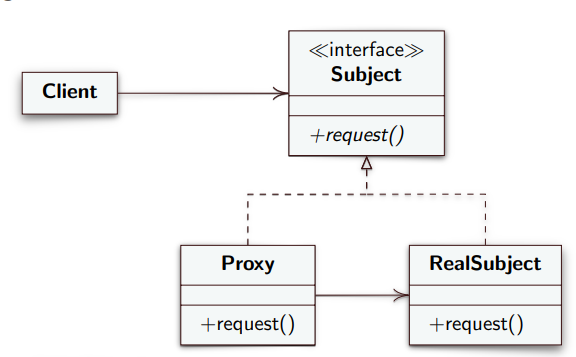
\includegraphics[width=0.6\linewidth]{Images/uml_proxy.png}
    \caption{Diagramma UML delle classi del design pattern proxy.}
    \label{fig:uml_classi_proxy}
\end{figure}

Come possiamo notare in Figura \ref{fig:uml_classi_proxy}, avremo un'\textbf{unica interfaccia} che viene implementata da Proxy e RealSubject in maniera tale che il client, pur comunicando con il Proxy, non si renda conto di questo livello di indirettezza.\footnote{È importante per far sì che il proxy non venga bypassato, nascondere, anche nella documentazione, il nome del RealSubject.} Sarà dunque il proxy, dopo aver eseguito eventuali controlli e/o operazioni, a inoltrare la richiesta al RealSubject. Un esempio di questo flusso di esecuzione è mostrato nella figura a seguire.

\begin{figure}[H]
    \centering
    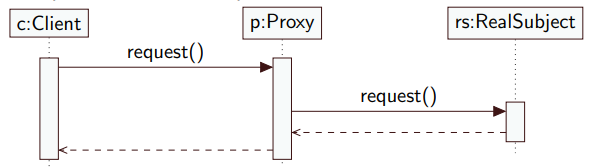
\includegraphics[width=0.8\linewidth]{Images/uml_sequenza_proxy.png}
    \caption{Il client effettua una richiesta al Proxy che la inoltra successivamente al RealSubject.}
    \label{fig:uml_sequenza_proxy}
\end{figure}


Quando questo pattern viene utilizzato per implementare politiche di protezione degli accessi ad oggetti, questo si dirà \textbf{Protection Proxy}. Un esempio è se si vuole concedere l'accesso in scrittura o in lettura, dei campi delle istanze di una classe Book in base ad un insieme di regole, per es. identità dell'utente che ne fa richiesta, libro richiesto, parte del libro, operazione richiesta.

\begin{figure}[H]
    \centering
    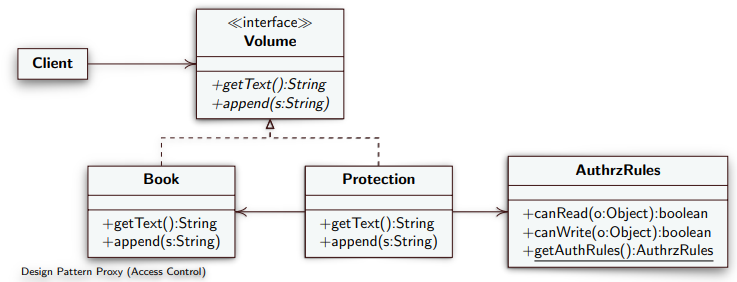
\includegraphics[width=0.8\linewidth]{Images/protection_proxy_uml.png}
    \caption{Esempio di UML delle classi per un Protection Proxy}
    \label{fig:protection_proxy_UML}
\end{figure}

\begin{figure}[H]
    \centering
    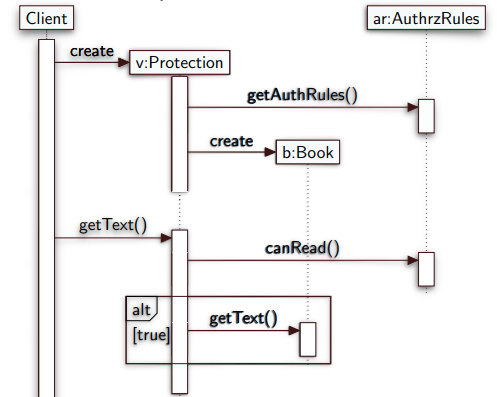
\includegraphics[width=0.6\linewidth]{Images/sequenza_protection_proxy.png}
    \caption{Flusso d'esecuzione del protection proxy}
    \label{fig:placeholder}
\end{figure}

Visto che questa per ogni RealSubject, serve un Proxy, è chiaro che questo pattern aumenti la proliferazione delle classi. Tuttavia, grazie all'indirettezza introdotta dalla classe Proxy, possiamo implementare potilitche di protezione degli accessi, cache per ottimizzare risultati di query onerose oppure per implementare meccanismi di \textbf{Copy-on-Write}, che consistono nell'utilizzo della stessa referenza ad un oggetto fino a quando non avvengono delle modifiche. Ad esempio, tornando all'esempio di prima, possiamo far sì che tutti i client facciano riferimento allo stesso libro fino a quando questo non viene modificato da un client che quindi creerà la sua copia.

In fine, un'altra variante utile potrebbe essere quella dei \textbf{Proxy Multipli}, per cui un proxy inoltra la richiesta ad un altro proxy e così via.

\section{Reference Monitor}
Al fine di sviluppare un sistema sicuro, è necessario rispettare dei requisiti di sicurezza oltre che quelli funzionali. L'obiettivo del reference monitor è quello di regolare gli accessi solo a certe condizioni e solo su certe risorse in maniera più completa rispetto a quanto si potesse fare con il protection proxy. Il pattern descrive come definire un'astrazione che intercetta le richieste e controlla la conformità con le autorizzazioni con il grande vantaggio  di poter avere delle decisioni complesse e set ben articolati di regole.
\begin{figure}[H]
    \centering
    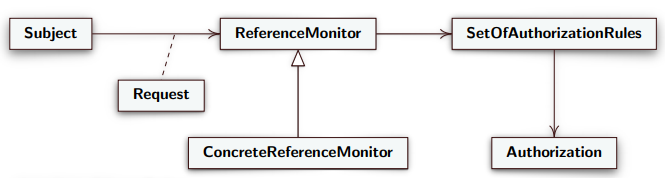
\includegraphics[width=0.8\linewidth]{Images/uml_reference_monitor.png}
    \label{fig:reference_monitor}
\end{figure}
Osservando in Figura, notiamo i seguenti oggetti:
\begin{itemize}
    \item \textbf{Protecion Object}: che rappresenta l'oggetto da proteggere;
    \item \textbf{Subject}: che richiede l'accesso all'oggetto protetto;
    \item \textbf{Request}: sarà l'effettiva richiesta da parte del subject;
    \item \textbf{Reference Monitor}: intercetta le richieste e cerca tra le regole l'autorizzazione che può essere usata sulla base della richiesta;
    \item \textbf{Conrete Reference Monitor}: implementa una specifica versione per un certo oggetto;
    \item \textbf{SetOfAuthorizationRules}: un insieme di regole di autorizzazione;
    \item \textbf{Authorization}: singola regola di autorizzazione.
\end{itemize}
Possiamo notare da qui anche la differenza tra il reference monitor e il proxy. Infatti, se il proxy implementa la stessa interfaccia dell'oggetto reale, qui abbiamo un vero e proprio intermediario che può o non può nascondere l'oggetto reale. Request è una classe che si interfaccia tra il soggetto e l'oggetto protetto e in un qualche modo li collega. Tipicamente la request è una classe che contiene attributi che caratterizzano la richiesta e che poi saranno utilizzate per cercare la regola adatta.
\begin{figure}
    \centering
    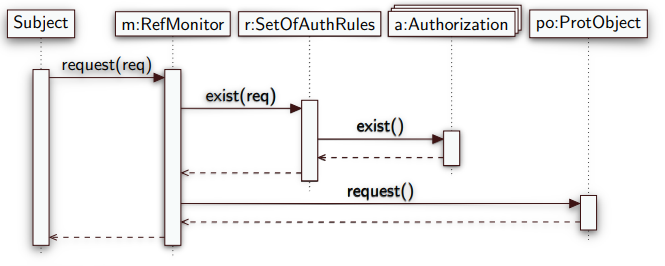
\includegraphics[width=0.8\linewidth]{Images/sequenza_reference_monitor.png}
    \label{fig:seq_reference}
\end{figure}

Anche in questo caso se tutte le richieste sono intercettate, possiamo imporre diverse regole di accesso sulla base di ciò che più vogliamo. Tuttavia, i controlli potrebbero rallentare le prestazioni, per cui può essere più utile effettuare \textbf{un solo controllo} per esempio all'apertura sul file piuttosto che per ogni operazione oppure mantenere una sorta di cache per le richieste più costose o più frequenti.

\section{Pattern Role-Based Access Control}
Come i precedenti pattern, l'obiettivo è quello di voler dare i diritti in base alle funzioni del proprio lavoro o dei compiti assegnati. Il problema è che in una grossa struttura con tante figure professionali, è difficile dare a tutti i permessi per le varie funzioni e tenere traccia di chi ha quale permesso. Generalmente si utilizza la regola \textbf{need-to-know policy} per cui ogni utente ha solo i diritti di accesso per le informazioni di cui necessita il suo ruolo.

La soluzione a questo problema è definire una classe utente e definire separatamente i ruoli che possono avere dei certi permessi su degli oggetti protetti. Questi ruoli saranno mappati in un oggetto o comunque da qualche parte per tenere traccia di quale utente ha quale ruolo attivo.
\begin{figure}[H]
    \centering
    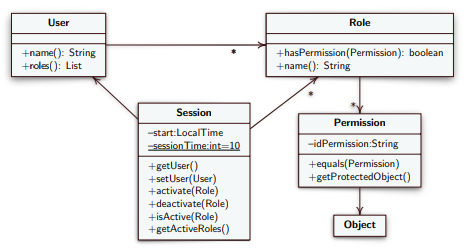
\includegraphics[width=0.8\linewidth]{Images/uml_rbac.png}
    \label{fig:uml_rbac}
\end{figure}
\begin{figure}[H]
    \centering
    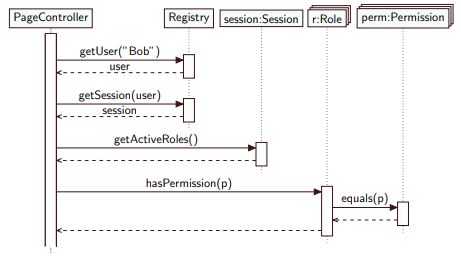
\includegraphics[width=0.8\linewidth]{Images/sequenza_rbac.png}
    \label{fig:sequenza_rbac}
\end{figure}

Questo pattern naturalmente necessita di un altro meccanismo parecchio importante che è quello di \textbf{autenticazione} che vedremo più avanti. Nel mentre, possiamo dire che questo pattern permette agli amministratori di gestire la complessità della sicurezza e dei ruoli in maniera molto più semplice. Inoltre, si potranno anche organizzare i ruoli in maniera più comoda anche nel sistema stesso e nel momento in cui si aggiunge un nuovo utente sarà possibile assegnare in maniera molto semplice i ruoli.

\section{Authenticator}
L'obiettivo di questo pattern è permettere di verificare che il soggetto che intende accedere al sistema è chi dice di essere. Ciò è dovuto al fatto che sistemi software contengono risorse che possono avere un certo valore e/o che per motivi vari, hanno dei limiti alle persone che vi possono accedere. 

Abbiamo quindi la necessità di garantire accesso con:
\begin{itemize}
    \item \textbf{Flessibilità}: una varietà di utenti richiede accesso al sistema e vi sono una varietà di parti, ciascuna con risorse a diversi livelli di riservatezza.
    \item \textbf{Dependability}: necessitiamo di autenticare gli utenti in modo affidabile e sicuro.
    \item \textbf{Costo}: abbiamo bisogno di un accesso che sia un buon compromesso tra sicurezza e costo, sia in termini di denaro che in termini di \textbf{prestazioni} nel caso in cui si debbano fare molti accessi.
    \item \textbf{Frequenza}: idealmente, vorremo far sì che i soggetti non debbano autenticarsi in maniera frequente così da migliorare l'esperienza dell'utente.
\end{itemize}
Per risolvere questi problemi, ciò che faremo sarà utilizzare un \textbf{singolo punto di accesso} che riceve le interazioni di un
soggetto con il sistema e applicare un protocollo per verificare l’identità del soggetto. Un esempio di singolo punto di accesso è quello al sistema operativo, non chiediamo l'accesso a ogni singola cartella, bensì chiediamo le credenziali solo all'accensione del SO. La soluzione avrà dunque la seguente struttura:
\begin{figure}[H]
    \centering
    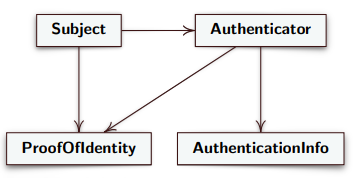
\includegraphics[width=0.5\linewidth]{Images/uml_autenticathor.png}
\end{figure}
Dove il soggetto richiede l'accesso, se questo va' a buon fine, allora al soggetto viene rilasciato dall'Authenticator una \textbf{ProofOfIdentity} che garantisce che il soggetto è chi dice di essere. Per verificare che l'utente è chi dice di essere, l'Authenticator chiama Verify su Authenticationinfo che verifica ciò che l'utente ha inserito. Vedremo più che, generalmente, la ProofOfIdentity non è altro che un \textbf{Token}.
Questo pattern ci garantisce:
\begin{itemize}
    \item Flessibilità: poiché possiamo gestire separatamente i modi di autenticazione degli utenti.
    \item Dependability: poiché le informazioni sono separate dall'autenticazione in sé, le possiamo memorizzare in aree protette.
    \item Costo: possiamo usare vari modi per autenticarci e in base a questi, si decide il costo. Di solito si sceglie tra password, id card e biometria.
    \item Performance e frequenza: il fatto che all'utente venga rilasciato un token, fa' sì che questo non debba per forza autenticarsi ogni volta che acceda a un servizio di un dato ecosistema. 
\end{itemize}

Le password degli utenti non possono e non devono essere mai in chiaro, bensì conserveremo un derivato della password che è l'Authenticationinfo. In genere, questo derivato è il risultato di una funzione Hash applicata alla password. Queste funzioni sono \textbf{deterministiche, irreversibili, con lunghezza fissa} e, inoltre, sono sensibili al \textbf{minimo cambiamento al messaggio} che genera Hash completamente diversi. In generale, per evitare brute force di password, usiamo \textbf{funzioni hash lente} così da rallentare anche un eventuale attaccante. Inoltre, per evitare l'utilizzo di rainbow table si utilizza anche il \textbf{salt} così da rendere le password ancora più lunghe di quanto non lo siano da standard. 

\subsection{Rate-Limiting}
Al fine di evitare attacchi di tipo \textbf{DoS} e \textbf{DDoS} che mirano a rallentare o far crollare completamente un servizio, si preferisce andare a utilizzare un rate-limiter che non fa' altro che dare un massimo di richieste che il sistema può gestire in un certo tempo. Così facendo, evitiamo che un singolo utente bombardi il nostro servizio di richieste che il nostro sistema, usando risorse per rispondergli, non potrà dedicarsi ad altro e ad altri. 

Questo limiter può essere inserito al livello del reverse proxy o a gateway di accesso al lato server prima che arrivino troppe richieste. 

\section{Token}
Come dicevamo, in un sistema distribuito vi possono essere più servizi al suo interno che, a loro volta, hanno bisogno che solo utenti autenticati e autorizzati li possano usare. Come dicevamo, un buon modo per far sì che l'utente non debba necessariamente autenticarsi per ogni servizio utilizzato, è quello di fornire una prova di autenticazione che sarà proprio il \textbf{Token}. Il sistema di Token funziona nel seguente modo:
\begin{figure}[H]
    \centering
    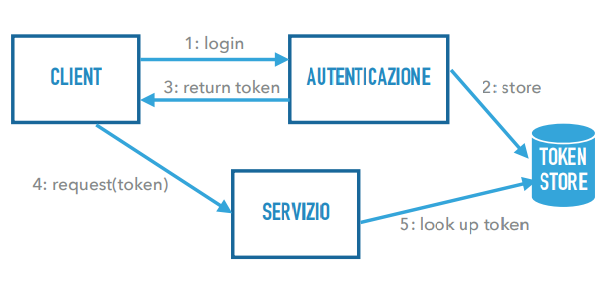
\includegraphics[width=0.5\linewidth]{Images/autenticazione_token.png}
\end{figure}
Come possiamo notare, una volta che l'utente si sarà autenticato al sistema, a questo viene fornito un token come prova di autenticazione che l'utente fornirà ogni qualvolta un servizio si chiederà se questo possa accedere o meno a esso. Il servizio per verificare che l'autenticazione sia ancora valida, farà riferimento a un \textbf{Token Store} che gli fornirà le informazioni necessarie a capire se l'utente può o non può accedere al sistema.

I token possono essere sotto forma di \textbf{stringhe} incomprensibili o, come tipicamente accade nella maggior parte dei casi, sotto forma di \textbf{oggetti} come ad esempio, i JWT. I token tipicamente indicano: ’utente identificato, chi lo ha emesso, il timestamp al momento dell’emissione, la durata, payload, una signature.
\subsection{JSON Web Token}
I JWT sono un formato standard per token di sicurezza che si basano su un set di \textbf{claim} per un utente. I JWT sono protetti crittograficamente e possono essere criptati.
Per evitare che chiunque crei il token o modifichi gli attributi del token, si aggiunge una \textbf{firma digitale} calcolata in base a una chiave segreta.

\section{Remote Proxy}
Nella variante di Remote Proxy, il client necessita di accedere a servizi di un componente che risiede su un altro host.
Il problema è che l’accesso diretto da parte del client all’oggetto remoto non è molto sicuro. I client non dovrebbero conoscere gli indirizzi di rete e i protocolli di comunicazione inter-processo. Inoltre, l'utente deve essere consapevole che è possibile vi siano ritardi nelle prestazioni causati da varie cose come magari reti congestionate o servizio lento a rispondere. È chiaro che una comunicazione con un host remoto sia molto più lenta rispetto che alla stessa comunicazione se l'host fosse in locale. 

Per risolvere questo problema, facciamo uso di un \textbf{Remote Proxy} che gestisce le richieste verso l'host remoto dove risiede il \textbf{Real Subject} che eseguirà le richieste. 
Sarà dunque il Remote Proxy a tenere la posizione in termini di IP e porta del real subject e implementerà ciò che è necessario per far comunicare le due macchine e i due processi.
Supponiamo di avere questo programma:
\begin{figure}[H]
    \centering
    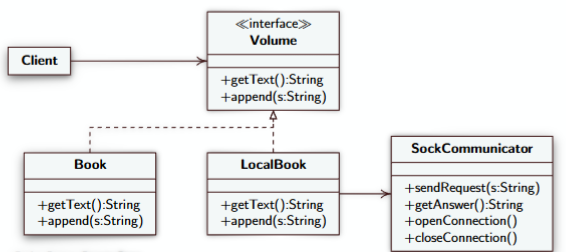
\includegraphics[width=0.7\linewidth]{Images/Remote_Proxy/uml_ex.png}
\end{figure}
Avremo che:
\begin{figure}[H]
    \centering
    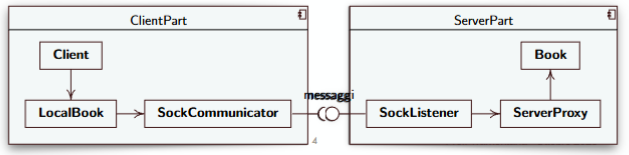
\includegraphics[width=0.7\linewidth]{Images/Remote_Proxy/diagramma_distribuito.png}
\end{figure}
\begin{itemize}
    \item \textbf{RemoteProxy(LocalBook)}: traduce chiamate a metodi in messaggi, inviati tramite SockCommunicator, e implementa il protocollo di comunicazione con l'altra parte.
    \item \textbf{SockCommunicator}: fornisce un’astrazione per la comunicazione, semplificando il RemoteProxy e permette di cambiare facilmente la tecnologia di comunicazione. Banalmente, se volessimo cambiare metodo di comunicazione, ci basterebbe solamente cambiare questa classe e implementare i metodi che il RemoteProxy chiama adattandoli al nuovo contesto. Vedremo a breve un pattern che fa' proprio questo.
    \item \textbf{SockListener}: viene avviato sull’host server per mettersi in ascolto di possibili messaggi che arrivano dalla rete.
    \item \textbf{ServerProxy}: traduce i messaggi appena arrivati lato server in chiamate a Book.
\end{itemize}

\section{Forwarder-Receiver}
Il design pattern Forwarder-Receiver fornisce comunicazione trasparente fra processi per sistemi che interagiscono tramite il modello peer-to-peer. Introduce \textbf{forwarder} e \textbf{receiver} per disaccoppiare i client dai meccanismi di comunicazione sottostante.
Nello sviluppo di applicazioni distribuite si usano meccanismi di
comunicazione fra processi come TCP/IP, socket, code di messaggi
Ciò che vogliamo è che:
\begin{itemize}
    \item Il sistema possa cambiare meccanismi di comunicazione senza dover modificare il client.
    \item Il mittente deve solo conoscere il nome dei ricevitori e nient'altro.
    \item La comunicazione tra i vari client non deve avere un impatto notevole sulle performance. 
\end{itemize}

Per risolvere questo problema, i peer collaborano e un peer può agire da client (richiede un servizio), o da server (fornisce un servizio), o entrambi. I \textbf{dettagli del meccanismo di comunicazione sottostante sono nascosti} ai peer, e incapsulati in componenti separati. Il pattern sarà quindi composto dai seguenti componenti:
\begin{itemize}
    \item \textbf{Peer}: sono responsabili dei compiti dell’applicazione e inviano messaggi ad altri peer o ricevono messaggi da altri peer.
    \item \textbf{Forwarder}: invia messaggi verso altri processi e fornisce un particolare meccanismo di comunicazione. Contiene il mapping fra nomi e indirizzi fisici. Nel messaggio trasmesso include il nome del proprio peer, così che il peer remoto possa inviare una risposta a esso.
    \item \textbf{Receiver}: sono responsabili di ricevere messaggi. Un receiver offre una interfaccia per uno specifico meccanismo di comunicazione IPC.
\end{itemize}
Un esempio di come viene utilizzato questo pattern è stato mostrato nella sezione precedente in cui si parlava del RemoteProxy. Usando entrambi i pattern Remote Proxy e Forwarder-Receiver si disaccoppiano meglio client, proxy e meccanismi di comunicazione. Per il pattern Remote Proxy, il RemoteProxy deve tenere la locazione del
RealSubject. Mentre, per il pattern Forwarder-Receiver, il Peer deve conoscere il nome del Peer destinatario, non la posizione. In genere, si preferisce far sì che il si conoscano solo il nome dei vari peer. Possono esserci vari tipi di messaggi:
\begin{itemize}
    \item \textbf{Messaggi Comandi}: che istruiscono il ricevente per fare qualcosa.
    \item \textbf{Messaggi informativi}: che contengono dati.
    \item \textbf{Messaggi Risposta}: che permettono di mandare una ricevuta per un messaggio ricevuto.
\end{itemize}

\section{Strategie di Distribuzione}
Le classi di un’applicazione potrebbero essere distribuite, in modo che ciascun oggetto sia posizionato su un suo host. Poiché le chiamate remote sono lente, è meglio combinare in una chiamata remota varie operazioni. Un oggetto locale ha un’interfaccia \textbf{fine-grained}, segue il principio generale OO di combinare piccole parti e rifinirle in vari modi per estendere la progettazione. Invece, l’interfaccia per un oggetto remoto è \textbf{coarse-grained} per far sì che non vengano effettuate tante chiamate remote come può accadere in locale.
Si preferisce quindi distribuire:
\begin{itemize}
    \item Inserendo le classi che lavorano insieme nello stesso processo.
    \item Replicando lo stesso processo su più host se è necessario gestire più cose.
\end{itemize}
Un classico esempio è quello di separare \textbf{client e server} o \textbf{server e database} dato che, in genere, compiono cose e sono progettate a scopi diversi. In generale, per progettare un sistema distribuito usando oggetti fine-grained bisogna:
\begin{itemize}
    \item Usare oggetti fine-grained internamente allo stesso host.
    \item Mettere oggetti coarse-grained ai confini della distribuzione, il cui solo scopo è fornire un’interfaccia remota a oggetti fine-grained.
    \item Gli oggetti coarse-grained agiscono da Facade per oggetti fine-grained. I \textbf{Remote Facade} minimizzano le difficoltà create da interfacce coarse-grained.
    \item Per trasferire coarse-grained object usare i \textbf{Data Transfer Object}.
\end{itemize}

\subsection{Remote Facade}
L'obiettivo è quello di fornire una facciata coarse-grained su oggetti fine-grained per migliorare l’efficienza sulla rete. Questo risolve il problema della lentezza delle chiamate remote a fine-grained object. Oggetti remoti che presentano interfacce coarse-grained permettono di minimizzare le chiamate ma complicano gli oggetti rendendo il codice meno chiaro. 
Infatti, il remote facade non fa' alto che tradurre metodi coarse-grained in oggetti sottostanti fine-grained. Tipicamente, un Remote Facade sostituisce i vari metodi get e set con un solo metodo get e un solo metodo set, chiamati \textbf{bulk accessors}.
\begin{figure}[H]
    \centering
    
\includegraphics[width=0.5\linewidth]{Images/Remote_Facade/uml.png}
\end{figure}
Per trasferire informazioni in grandi quantità occorre avere altri oggetti a supporto, ad esempio, se  il tipo restituito da getAddressData() è noto ad entrambi i lati della connessione ed è serializzabile, il metodo getAddressData() crea una copia dell’oggetto originale, altrimenti, è necessario utilizzare i così detti Data Transfer Object che vedremo a breve. 
Il remote Facade può anche avere altre responsabilità ad esempio può effettuare \textbf{controlli di sicurezza} e si possono anche applicare controlli di gestione per le \textbf{transazioni}\footnote{Qui si riferisce alle transazioni atomiche, cioè transazioni che iniziano e finiscono senza la possibilità che rimangano a metà.}. Un
metodo del facade può avviare la transazione, fare il lavoro interno, quindi fare commit alla fine. 
\subsection{Data Transfer Object}
Quando si lavora con un'interfaccia remota, ogni chiamata ha un certo costo e, per ridurre il numero di chiamate, spesso si preferisce più dati a ogni chiamata. Per far risolvere questo problema si utilizzano i \textbf{Data Transfer Object (DTO)} che tiene tutti i dati della chiamata. Questo oggetto deve essere \textbf{serializzabile} cioè deve implementare l'interfaccia Serializable che permette la trasformazione dell'oggetto in una sequenza di Byte per salvarlo su disco. 

Un DTO è un oggetto che ha vari campi e metodi getter e setter. I suoi campi sono dati primitivi e classi semplici così da rendere la sua struttura semplice. Il DTO porta i dati che l'oggetto remoto ha chiesto e spesso possono esserci più DTO corrispondenti a richieste diverse e alle risposte.

Oltre che ai veri metodi di accesso, il DTO è responsabile della sua serializzazione in qualche formato come ad esempio in binario o in XML. In genere, si preferisce quest'ultima alla serializzazione in binario poiché un minimo cambiamento fa' sì che la serializzazione in binario non sia più la stessa, di fatto, rendendo incompatibili DTO di versioni diverse. Vediamo un esempio:
\begin{figure}[H]
    \centering
    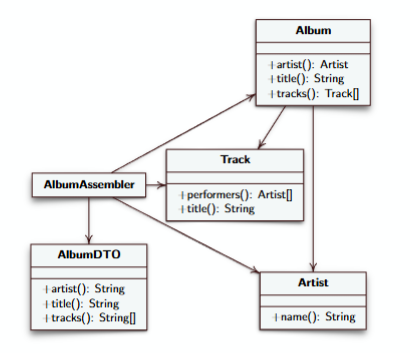
\includegraphics[width=0.5\linewidth]{Images/Remote_Facade/DTO_ex.png}
\end{figure}

\subsection{Remote Method Invocation}
Per far avvenire la comunicazione fra client e server si definisce una interfaccia Java comune a entrambi i due lati, Per il codice di esempio del Remote Facade, tale interfaccia è AlbumService, e contiene la definizione dei metodi che vogliamo far usare al client. 
Per RMI, l’interfaccia deve essere un sottotipo dell’interfaccia \textbf{java.rmi.Remote}. Vedremo che \textbf{lato client}, Per localizzare un oggetto che esiste in remoto si usa un’operazione di lookup attraverso un identificatore sul servizio di \textbf{Naming} (ovvero RMI registry). Questa operazione fornirà un proxy per accedere all’oggetto remoto.
\textbf{Lato server}, invece, si crea un oggetto, si registra l’oggetto sul servizio di Naming. 
\begin{figure}[H]
    \centering
    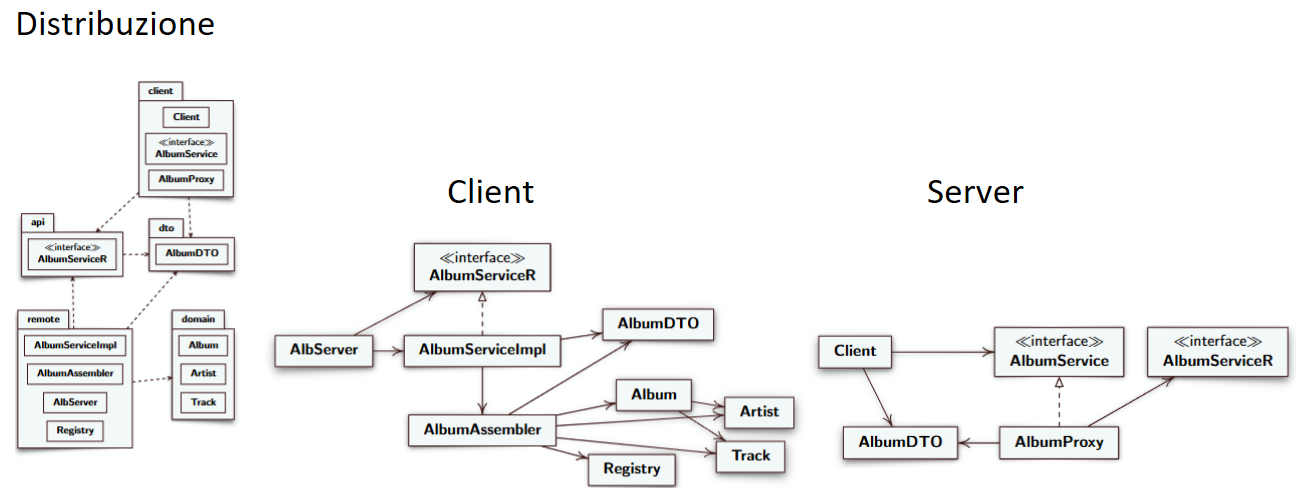
\includegraphics[width=1\linewidth]{Images/Remote_Facade/RMI.png}
\end{figure}
Quello che accadrà sarà, quindi, che il client contatterà RMI chiedendo di utilizzare un servizio e questo gli fornirà un Proxy che il client utilizzerà come se fosse l'oggetto reale.È importante sottolineare che ogni chiamata a metodo che fa' uso di RMI lancia un eccezione di tipo RemoteException poiché potrebbe non andare a buon fine.

\section{Sessione}
Una sessione è un'interazione a lungo termine fra un client e un server. Può consistere di una singola richiesta o di una serie di richieste. Tipicamente una sessione inizia quando un utente fa login, e termina quando l’utente fa logout o semplicemente va via. Le sessioni o server possono essere:
\begin{itemize}
    \item \textbf{Stateless}: Se non si conservano i dati prodotti tra una sessione e l'altra.
    \item \textbf{Stateful}: Il server tiene traccia di ciò che il client di un certo IP ha fatto.
\end{itemize}

È chiaro che un server stateful consumi più risorse rispetto a un server stateless poiché necessita di utilizzare delle risorse solo per mantenere ciò che è accaduto nelle precedenti sessioni. Un server che ha tanti utenti dovrebbe essere stateless, per evitare un enorme consumo di risorse, tuttavia, è chiaro che il fatto che una sessione sia stateful sia molto più comodo per gli utenti.

Innanzitutto, i \textbf{dati di sessione} vanno distinti dai \textbf{dati permanenti} che devono essere convervati e disponisbili per tutte le sessioni. Per gestire lo stato della sessione esistono diversi approcci basati su \textbf{client, server o database}.

\subsection{Client Session State}
In questo caso, il nostro obiettivo sarà quello di conservare lo stato della sessione sul client. Per fare ciò, faremo in modo che tutti i dati della sessione siano sul client e sarà lui stesso a mandarli con ogni richiesta al server e il server, a ogni risposta, li reinvierà ogni volta. Per realizzare questo sistema possiamo utilizzare un \textbf{DTO}, oppure, in caso di HTML, possiamo utilizzare \textbf{parametri URL, campi nascosti e cookie}:
\begin{itemize}
    \item \textbf{Sessione URL}: con pochi dati può funzionare bene e l'associazione di un ID di sessione può essere fatta in automatico dalla piattaforma cambiando l'URL.
    \item \textbf{Campi Nascosti}: Un campo nascosto è un campo inviato al browser ma non visualizzato sulla pagina web. Lo stato della sessione è inserito in un campo nascosto e serializzato con la risposta. XML può essere usato come formato per i dati inseriti nel campo nascosto.
    \item \textbf{Cookie}: I cookie vengono inviati in maniera automatico, tuttavia se l'utente li disattiva, il sito non funzionerà correttamente. Inoltre, un cookie funziona solo per un singolo nome di dominio, quindi siti separati in diversi nomi di dominio non vedranno i cookie di altri siti.
\end{itemize}
Questa cosa funziona bene insieme a server object stateless, e riesce a far recuperare la sessione quando un server va giù e viene sostituito.Si usa quasi sempre per identificare la sessione. Per evitare che qualcuno catturi una sessione di un altro (cambiando l’ID di sessione) si usa l’hash di un ID semplice.
Tuttavia, Con grandi quantità di dati, il tempo di trasferimento durante una richiesta può diventare proibitivo e i dati inviati al client possono essere visti e alterati, i dati rinviati al server devono essere riconvalidati. Il criptaggio e decriptaggio a ogni richiesta può essere un problema per le prestazioni.
\begin{figure}[H]
    \centering
    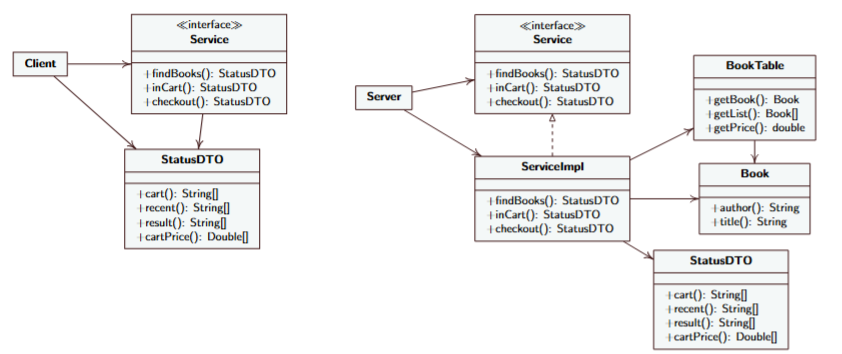
\includegraphics[width=0.9\linewidth]{Images/Sessione/client_dto.png}
\end{figure}

\subsection{Server Session State}
Un oggetto di sessione può essere tenuto in memoria sul lato server dell'applicazione. Una mappa in memoria tiene il riferimento a oggetti di sessione tramite la chiave pari all’ID di sessione. Dall’ID si prende l’oggetto dalla mappa e si può servire la richiesta del client. 
Per risolvere il problema della memoria limitata, si serializza lo stato dell'oggetto sessione  si immagazzina su uno storage, ovvero l’oggetto di sessione è \textbf{passivato}.\footnote{Cioè viene salvato su disco e tolto dalla memoria.}
Lo storage può essere il \textbf{file system} o un \textbf{database}. Lo storage, se gestito separatamente rispetto agli host, è possibile ottenere:
\begin{itemize}
    \item \textbf{Clustering}: cioè possiamo distribuire richieste a più server.
    \item \textbf{Failover}: se un host va giù il controllo va' a un altro server che può recuperare tranquillamente i dati. 
\end{itemize}
Il punto di forza è la semplicità, se vi è sufficiente memoria, tuttavia clustering e failover possono essere complicati da gestire.
\begin{figure}[H]
    \centering
    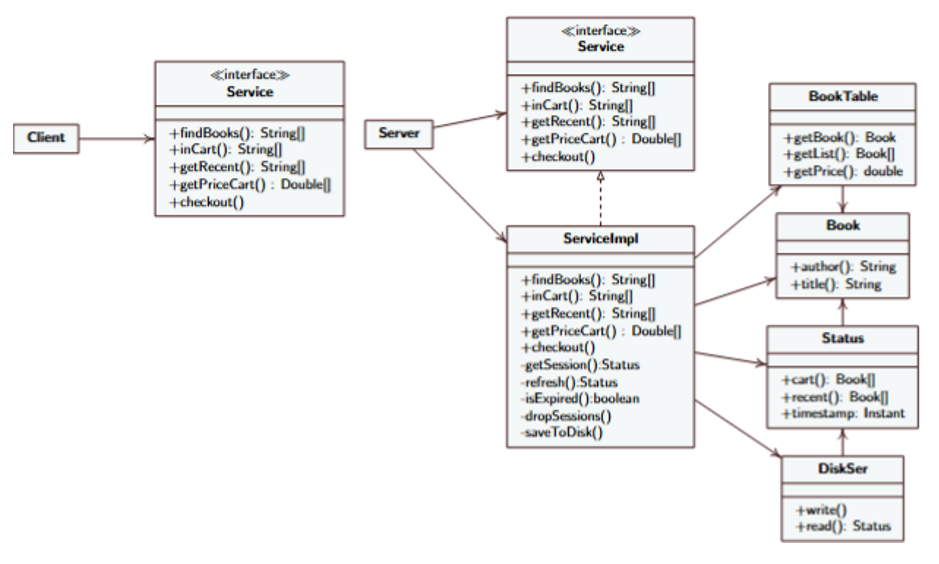
\includegraphics[width=0.8\linewidth]{Images/Sessione/server.png}
\end{figure}

\subsection{Database Session State}
Quando una richiesta del client arriva sul server, anzitutto il server prende i dati necessari dal database. Per riprendere i dati della sessione è necessario almeno un ID di sessione che è conservato sul client. I dati di sessione devono essere considerati locali, e altre parti
del sistema non dovrebbero usarli, fino a quando non si fa commit della sessione.

I dati di sessione conservati sul database devono essere considerati dati intermedi e distinti dagli altri che sono stati confermati. Per fare ciò, può essere utile aggiungere un nuovo campo booleano \textbf{pending} che ci dice se il dato è temporaneo o è definitivo. Inoltre, possono essere utilizzate delle \textbf{tabelle separate} solo per i dati di sessione. Tipicamente ci sono regole per la convalida dei dati conservati sul database che assicurano l’integrità dei dati. Tali regole non vanno applicate ai dati pending, che invece potrebbero necessitare di altre regole. Avere tabelle separate facilita l’applicazione di regole diverse

Le tabelle di dati pending dovrebbero essere \textbf{clonate dalle tabelle reali}, ovvero stessi nomi di campi fra le due tabelle, e un campo aggiuntivo per le tabelle pending per l’ID di sessione. 

Se una sessione è cancellata l’ID di sessione permette di trovare tutti i
dati da cancellare, oppure se la sessione è abbandonata, si può usare un timeout, un \textbf{daemon} esegue a intervalli di pochi minuti per trovare e \textbf{cancellare i vecchi dati}.

E’ necessario del tempo per l’accesso ai dati per ciascuna
richiesta. Una cache può ridurre questi tempi La programmazione della gestione dello stato della sessione può essere semplificata non tenendo lo stato in memoria, ma conservandolo sul database.

\subsection{Serialized LOB}
La serializzazione può essere fatta in binario (BLOB) o come caratteri (CLOB). Un oggetto serializzato è un \textbf{oggetto rappresentato come una sequenza di byte} che include i dati dell’oggetto e informazioni sul tipo dell’oggetto e sui tipi di dati conservati nell’oggetto. Quando si usa il Serialized LOB bisogna fare attenzione ai problemi di duplicazione di dati poiché lo stesso oggetto potrebbe essere salvato per due contesti diversi.
Se nel grafo da memorizzare, a partire dall’oggetto passato a writeObject() di ObjectOutputStream, si incontrasse un riferimento a un oggetto la cui classe non implementa Serializable si avrebbe un errore a runtime. Se si vuol escludere dalla memorizzazione un campo di un oggetto del grafo, il campo dovrà essere dichiarato transient. Se un campo che è il riferimento a un oggetto è dichiarato \textbf{transient}, la corrispondente classe non necessita di essere Serializable.

\section{Memento}
Alcune volte è necessario \textbf{registrare lo stato interno di un oggetto}.Questo è richiesto quando si implementano i meccanismi di checkpoint e di undo che permettono di ritornare da operazioni non riuscite o ripristinare il sistema da situazioni di errore.Tuttavia, gli oggetti normalmente incapsulano il loro stato rendendolo inaccessibile ad altri oggetti e quindi impossibile salvarlo esternamente
Esporre lo stato \textbf{violerebbe l’incapsulamento}, e questo può compromettere l’affidabilità e l’estensibilità.

Dunque, per ovviare a questo problema utilizziamo il \textbf{memento}, cioè un oggetto che immagazzina una copia dello stato interno di un altro oggetto detto \textbf{originator} Il meccanismo di undo richiederà un memento all’originator quando è necessario avere un checkpoint dello stato dell’originator. L’originator imposta il memento con i dati che caratterizzano il suo stato corrente e solo l’originator può immagazzinare e riprendere informazioni dal memento.
\begin{figure}[H]
    \centering
    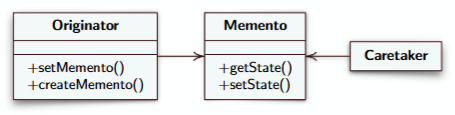
\includegraphics[width=0.8\linewidth]{Images/Memento/uml.png}
\end{figure}
Dunque, avremo che: 
\begin{itemize}
    \item \textbf{Memento}:  immagazzina lo stato interno dell’oggetto Originator, quali dati sono necessari è una scelta dell’Originator; protegge da accessi di altri oggetti diversi dall’Originator. Solo all’Originator è permesso l’accesso allo stato interno del Memento.
    \item \textbf{Originator}:crea un Memento che contiene una copia del suo stato interno; usa il Memento per ripristinare il suo stato interno.
    \item \textbf{Caretaker}: è responsabile di tenere il Memento; non usa o esamina il contenuto del Memento.
\end{itemize}

Semplifica l’Originator in quanto non deve tenere diverse versioni del suo stato che i client hanno chiesto di salvare. Se si chiede di copiare una grande quantità di informazioni o la richiesta di salvataggio dello stato avviene spesso, le prestazioni possono deteriorarsi.

\section{Idempotent Receiver}
Una operazione si definisce \textbf{idempotente} se questa può essere eseguita tante volte con lo stesso effetto che avrebbe se venisse \textbf{eseguita una sola volta}.

Molti sistemi usano il pattern “at-least-once delivery”, ovvero un messaggio è mandato non esattamente una volta ma almeno una volta per garantire affidabilità e ridurre i tempi di attesa, di conseguenza la ricezione duplicata è inevitabile. Dunque, immaginando un servizio di pagamento, se questo manda due volte il messaggio di pagamento, allora l'operazione verrà eseguita più volte se il sistema non è idempotente.

Dunque, il nostro obiettivo è quello di identificare le richieste dei client univocamente così da poter ignorare le richieste duplicate quando il client ritenta. Questo è necessario poiché Il client potrebbe mandare una richiesta ma non ricevere una risposta; per il client è impossibile sapere se la risposta è andata persa, o il server si è bloccato prima di elaborare la richiesta, dunque ritenta.

Quello che facciamo è una cosa di questo tipo:
\begin{enumerate}
    \item  Il client crea un ID univoco per la richiesta per es. numerando la richiesta, o tramite hash dei dati che costituiscono la richiesta; oppure chiede al server di creare un ID della richiesta.
    \item Il server crea una sessione per immagazzinare le risposte alle richieste dei client registrati e traccia il tempo dell’ultimo accesso del client.
    \item Quando il server riceve una richiesta, anzitutto controlla se la richiesta con quell’ID e da quel client è stata già elaborata. Se il server trova la richiesta conservata manda la stessa risposta al client altrimenti elabora la richiesta e ne conserva il risultato.
\end{enumerate}
Le richieste già elaborate e conservate potrebbero essere
\textbf{cancellate dal server dopo un timeout} o potrebbero essere numerate in modo progressivo e il server può quindi rimuovere le richieste salvate con numero minore rispetto a quella appena ricevuta.

Avremo quindi due componenti:
\begin{itemize}
    \item \textbf{MessageReceiver}: riceve e valida il messaggio, elabora il messaggio solo se non ancora gestito.
    \item \textbf{MessageDB}: conserva l’ID dei messaggi già elaborati.
\end{itemize}
Naturalmente, questo sistema ci garantisce l'effetto desiderato, tuttavia, abbiamo una maggiore occupazione della memoria per il salvataggio degli ID delle operazioni e un tempo di esecuzione più lungo dovuto alla gestione delle richieste scadute o comunque della gestione degli ID. 

\section{Request Batch}
Quando vi sono numerose richieste di piccole dimensioni, queste possono occupare molta banda in rete causando quindi un dispendio in termini di risorse. Dunque, per ridurre la \textbf{latenza} e l'\textbf{overhead} causate da un gran numero di piccole richieste, cerchiamo di \textbf{inviare più richieste aggregate in un batch}. Dunque, il client o un proxy accumula le richieste per un breve intervallo o fino a un numero massimo. La quantità da accumulare può essere determinata in base alla quantità di dati da inviare e ricevere quindi per usare meglio la banda di rete.
Il batch è inviato come un’unica richiesta al server. Il ricevente disaggrega il batch di richieste, processa le singole richieste, e restituisce le risposte in modo aggregato che saranno poi disaggregate e smistate ai richiedenti originali.

Avremo quindi le seguenti componenti:
\begin{itemize}
    \item \textbf{Request Sender}: raccoglie le richieste individuali.
    \item \textbf{Batch Assembler}: aggrega più richieste in un batch.
    \item \textbf{Batch Processor (Receiver)}: elabora il batch e produce le risposte corrispondenti.
    \item \textbf{Response Splitter}: distribuisce le risposte ai client originali.
\end{itemize}

Grazie a questo pattern riduciamo il numero di messaggi e, quindi, il \textbf{round-trip} e miglioriamo il \textbf{throughput} e l'utilizzo di risorsse. Tuttavia, introduciamo una \textbf{latenza di accumulo} procurata dal fatto che le richieste vengono aggregate prima di essere inviate. 

\section{Leader And Followers}
Per ottenere la \textbf{fault tolerance} in sistemi che gestiscono dati, i dati devono essere replicati su più server. Ciò implica che abbiamo la necessità di garantire consistenza dei dati ai client. Un \textbf{Majority Quorum} non è sufficiente, poiché in alcuni scenari di fallimento dei server i client vedrebbero dati inconsistenti. Solo quando i dati sono letti da più server le inconsistenze possono essere risolte, ma a volte questo non basta. 

Immaginiamo di avere 3 server e che su uno viene fatto l'aggiornamento di un dato mentre sugli altri no. Quello che potrebbe accadere è che un client potrebbe leggere il dato sui due server su cui l'aggiornamento non è andato a buon fine, di fatto, leggendo un dato scaduto. 

Per risolvere questo problema selezioniamo un server come \textbf{Leader} e questo sarà responsabile di prendere decisioni per l'intero cluster e propagare le decisioni prese. Solo il leader gestisce le richieste dei client. Se una richiesta è mandata direttamente a un server che è un follower, questo la propaga al leader. 

Dunque, ogni server all’avvio cerca un leader, se non lo trova allora avvia una \textbf{elezione del leader} durante il quale, non si accettano richieste fino a che non viene eletto un leader. Un Leader può essere eletto secondo i seguenti criteri:
\begin{itemize}
    \item Il server con Generation Clock più recente può essere il leader.
    \item Se tutti i server sono equamente aggiornati, allora o si prende il server con \textbf{ID più alto}, o si prende il server che avvia \textbf{l'elezione per primo}.
\end{itemize}

A ogni elezione del leader si incrementa il numero \textbf{Generation Clock} che sarà una sorta di identificativo che servirà più avanti. Un server può essere solo in uno dei seguenti stati: \textbf{Leader, Follower e Candidate}.
Inoltre, per capire se il leader è ancora attivo, si utilizza un meccanismo detto di \textbf{Heart Beat}. 

\subsection{Heart Beat}
Quando più server formano un cluster, è importante accorgersi tempestivamente di un fallimento di un server per avviare azioni correttive rendendo un server responsabile per la gestione delle richieste dei dati che erano sul server non disponibile. 

Per fare ciò, viene inviata periodicamente un richiesta agli altri server detta \textbf{liveness} che sta a indicare agli altri la presenza del leader. Se questa non arriva entro un certo \textbf{timeout} che, solitamente, è un multiplo del round-trip, allora si lavora come se quel server non fosse più disponibile. Nel caso Leader e Followers, si inizia una nuova elezione. 

\subsection{Majority Quorum}
Con il Majority Quorum vogliamo ottenere:
\begin{itemize}
    \item \textbf{Liveness}: che è la proprietà di un sistema che dice che il sistema progredisce sempre.
    \item \textbf{Safety}: è la proprietà che dice che il sistema è sempre nello stato corretto. 
\end{itemize}
Quando un server aggiorna un dato, la replica del dato su altri server assicura che il dato sarà disponibile pur se il server fallisce. Con tante copie ci vorrà \textbf{più tempo per le conferme} e si riduce la liveness, troppe poche copie e \textbf{il dato potrebbe essere perso} e non si ha safety. 

Per risolvere questo problema, un cluster concorda di aver ricevuto un aggiornamento quando la maggioranza dei nodi del cluster conferma l'aggiornamento. Tale numero è detto \textbf{quorum} e, se un cluster ha n nodi, allora il quorum è $n/2+1$. 
Il quorum indica quanti fallimenti possono essere tollerati. Il numero di fallimenti tollerati è la dimensione del cluster meno il quorum.
Potremmo avere due quorum diversi per due operazioni diverse, ad esempio, posso voglio rendere più veloci le operazioni di lettura mentre posso volere più ridondanza sulle operazioni di scrittura. L'importante è che l'intersezione non sia vuota. Ad esempio, supponiamo di avere 5 nodi e che il quorum di lettura sia 2 mentre quello di scrittura sia 3. Quello che potrebbe accadere è che la scrittura va a buon fine su 3 nodi ma sugli altri due no. Dunque, se un client legge su quei due nodi che hanno il dato non aggiornato, allora il nostro intento fallisce. 

\subsection{Generation Clock}
In un contesto di Leader e Follower, c’è la possibilità che un leader sia temporaneamente disconnesso dai follower per mancanza di rete. Il processo del leader esegue ancora, e quando la rete ritorna disponibile il server manderà richieste di repliche ai follower. Tuttavia, nel cluster vi sarà un nuovo leader che quindi avrà un numero di generazione diverso rispetto al precedente.
Dunque, ogni nodo che riceve richieste da un leader con generazione più bassa rispetto a quella nuova, dovrà ignorare le richieste.

\section{Request Pipeline}
La comunicazione fra server di un cluster usando un singolo canale può causare problemi di prestazioni se le richieste devono aspettare le risposte delle precedenti richieste.  Per ottenere un migliore throughput, la coda di richieste sul server dovrebbe essere sufficientemente piena per far sì che la capacità del server sia pienamente usata. Se si manda solo una richiesta alla volta molta della capacità del server sarà sprecata.

I nodi mandano le richieste agli altri nodi senza aspettare le risposte alle precedenti richieste, per questo, si usano due thread separati uno per mandare le richieste su un canale di rete e un altro thread per
ricevere le risposte dal canale di rete. Il nodo ricevente elabora immediatamente la risposta o la \textbf{mette in una coda}.

Alcuni possibili problemi:
\begin{itemize}
    \item il nodo che accetta le richieste potrebbe essere \textbf{saturato}. Per questo motivo si mette un limite al numero di richieste inevase.
    \item Ogni nodo può mandare un massimo di richieste agli altri nodi. Al raggiungimento del limite, senza aver ricevuto risposte, il richiedente è inibito dal mandare richieste.
    \item Una coda può essere tenuta per le richieste non inviate. Una volta che una risposta viene ricevuta, questa libera una possibile richiesta che era in coda.
    \item La gestione dei fallimenti può essere difficile. Una prima richiesta che fallisce, potrebbe essere ritentata e una seconda richiesta potrebbe essere eseguita prima di ritentare la prima richiesta.
    \item Occorre un meccanismo per rifiutare le richieste fuori ordine. Un identificativo unico per richiesta, fornito dal lato server, permette di controllare l’ordine delle richieste
\end{itemize}
 

\section{Stabilità}
Una \textbf{transazione} è una certa unità di lavoro che un sistema elabora. Per esempio una transazione è “Un cliente fa un ordine” e questa operazione include tanto codice e persino l’integrazione con sistemi esterni per la verifica della carta di credito. Un sistema \textbf{resiliente} continua a elaborare transazioni persino quando ci sono guasti nei componenti che disturbano l’elaborazione. Questo è spesso inteso come \textbf{stabilità}. Non solo che server e applicazioni sono in esecuzione, ma che l’utente può svolgere del lavoro. 

\subsection{Timeout}
Oggi tutte le applicazioni non banali usano la rete in qualche modo, esponendo l’applicazione al possibile fallimento della rete. Quando ciò capita, il nostro codice non può aspettare indefinitamente una risposta che potrebbe non arrivare mai, prima o poi deve rinunciare. il timeout è un semplice meccanismo che permette di \textbf{smettere di aspettare} una risposta quando si sospetta che non arriverà. 

Ad esempio, Un pool di risorse che blocca i thread dovrebbe avere un timeout per assicurare che i thread siano sbloccati sia quando le risorse diventano disponibili che quando non lo diventano. Dunque, è sempre bene utilizzare funzioni wait o lock ecc. che utilizzano dei timeout come parametro. Un modo per gestire i timeout è organizzare operazioni che prendono molto tempo in un set di primitive che sono riusate in vari posti. Ad esempio, piuttosto che gestire una struttura composta di continui try catch per il collegamento a un db, creiamo una funzione collegaDB che si occupa di tutto e utilizziamo sempre quella che sa' già come gestire gli errori.

È importante ricordarsi che riprovare immediatamente potrebbe generare lo stesso problema, e lo stesso timeout. Il più delle volte si dovrebbe accodare l’operazione e riprovare dopo. 

\subsection{Circuit Breaker}
Il dispositivo di interruzione del circuito esiste per permettere a un sottosistema di fallire (per l’eccessiva corrente assorbita) senza distruggere l’intero sistema. Una volta che il pericolo è passato, il dispositivo di interruzione può essere reimpostato per ripristinare il pieno funzionamento del sistema.

Applicando la stessa tecnica sul software, si può schermare un’operazione pericolosa con un componente che evita le chiamate quando il sistema non funziona bene. Nello stato normale di \textbf{“chiuso”}, il circuit breaker esegue le operazioni. Queste possono essere chiamate a un altro sistema, o chiamate interne soggette a timeout o fallimenti. In questo caso possiamo avere due esiti:
\begin{itemize}
    \item Se la chiamata ha successo non succede niente di speciale.
    \item Se la chiamata fallisce, il circuit breaker prende nota, e una volta che un certo numero di fallimenti (o frequenza di fallimenti) eccede una soglia, il circuit breaker “apre” il circuito.
\end{itemize}
Quando il circuito è \textbf{“aperto”}, le chiamate al circuit breaker falliscono immediatamente senza alcun tentativo di eseguire l’operazione.
Dopo una certa quantità di tempo, il circuit breaker decide che l’operazione potrebbe riuscire e va nello stato di \textbf{“semi-aperto”} e dunque la prossima chiamata è abilitata a eseguire l’operazione a
rischio:
\begin{itemize}
    \item Se la chiamata ha successo il circuit breaker ritorna nello stato di “chiuso”.
    \item Se la chiamata fallisce il circuit breaker ritorna allo stato di “aperto”, fino allo scadere di un altro timeout.
\end{itemize}
I circuit breaker sono un modo per \textbf{degradare le funzionalità quando il sistema è sovraccarico}.I cambiamenti di stato del circuit breaker dovrebbero essere registrati nei \textbf{log}, e lo stato corrente dovrebbe essere mostrato in caso di monitoring.

\subsection{Bulkheads}
In una nave, le paratie sono barriere che possono essere chiuse per dividere la nave in compartimenti a tenuta. Le paratie prevengono che l’acqua si sposti da una sezione a un'altra. Così una singola falla nello scafo non affonda la nave. Questo sistema utilizza il principio di \textbf{contenimento del danno}, così facendo, partizionando un sistema software si può evitare che il fallimento in una parte distrugga tutto.

La ridondanza fisica è la forma più comune di paratia. Se ci sono server indipendenti, il fallimento di un hardware non coinvolge altri. Su larga scala, ci potrebbero essere varie farm di server, con alcune farm dedicate a parti mission-critical. Un sistema di biglietti potrebbe avere server dedicati per il check-in, questi non sono influenzati da altri che gestiscono query sullo stato dei voli, che potrebbero essere sovraccarichi da tante richieste.

Su scala più piccola, CPU binding è una forma di paratia. Fare il binding di un processo a una CPU evita che un processo fuori controllo usi tutti i cicli di CPU di tutte le CPU e tira giù tutta la macchina.

\subsection{Sistemi Reattivi}
I sistemi reattivi esibiscono Resilienza e si basano sulla Messagistica. Il sistema risponde in tempi appropriati sebbene in presenza di guasti. Ciò è ottenuto tramite repliche, contenimento, isolamento, e delega. I guasti sono isolati all’interno di un componente, in modo che parti che si guastano (bloccano) e si riavviano non compromettono l’intero sistema. 

Ci si affida ad un sistema di passaggio di messaggi asincroni per stabilire una connessione fra componenti che assicura un lasco accoppiamento, isolamento, e location transparency.

\section{Future}
L’interfaccia Future<V> permette di rappresentare un risultato (di tipo V) che sarà disponibile in un momento successivo (futuro). Rappresenta un compito che esegue in modo \textbf{asincrono} ed è un riferimento al risultato. L’avvio di un’attività per mezzo di un Future permette al thread chiamante di \textbf{continuare a fare del lavoro}, anziché aspettare il risultato dell’operazione.
\begin{figure}[H]
    \centering
    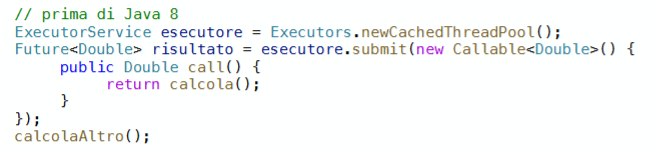
\includegraphics[width=0.7\linewidth]{Images/Future/future.png}
\end{figure}
Qui avremo che:
\begin{itemize}
    \item \textbf{submit()}: avvia un’operazione che ritorna un Future che rappresenta il risultato dell’operazione.
    \item \textbf{Executors e newCachedThreadPool()}: permettono di creare un nuovo thread, ovvero l’istanza di ExecutorService. Tale istanza esegue l’operazione richiesta.
    \item \textbf{ExecutorService}: è un’interfaccia che fornisce il metodo submit(), che prende in ingresso un Callable. Un Callable è un’interfaccia che dichiara il metodo call() che ritorna un risultato.
\end{itemize}

Quando non si può più procedere senza il risultato dell’operazione che prende tanto tempo e che sta eseguendo sul thread aggiuntivo, si può prendere il risultato chiamando get() sul Future ovvero sulla variabile risultato. Questo metodo restituirà il valore se presente altrimenti si blocca. Tramite overload, si può anche inserire un Timeout che impedisce al thread di aspettare all'infinito.

\subsection{CompletableFuture}
CompletableFuture permette di avviare esecuzioni parallele in modo conciso. Sia computePrice() un metodo che, accedendo a un servizio remoto, ha un tempo di esecuzione lungo, Double computePrice(String s): 
\begin{figure}[H]
    \centering
    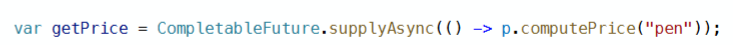
\includegraphics[width=0.8\linewidth]{Images/Future/varcompfuture.png}
\end{figure}
supplyAsync() è un metodo static che prende in ingresso un Supplier<U> cioè un interfaccia funzionale avente il metodo get che restituisce un tipo U. Questo metodo avvia un thread per eseguire il metodo get() del Supplier passato, e restituisce un nuovo CompletableFuture parametrizzato con U. Il Supplier verrà eseguito da uno dei thread degli Executors.

CompletableFuture get funziona esattamente come prima, estrae il valore se presente altrimenti aspetta. Questo metodo può lanciare eccezioni quando il thread è interrotto o quando viene generata un'eccezione. Inoltre, il metodo complete(T value) se non ha già completato l’esecuzione imposta il valore restituito poi da get() a value e ritorna True se il valore è stato impostato, altrimenti ritorna false.\footnote{Se ritorna false, vuol dire che c'era già un valore.} Esistono anche le versioni di queste operazioni con timeout. 

Un'altra cosa interessante è il \textit{thenApply()}, questo metodo si utilizza se si vuol usare il risultato di una prima esecuzione asincrona in un’altra esecuzione asincrona. La chiamata avviene in modo sincrono, ovvero non appena il risultato della prima esecuzione è disponibile.

Si abbiano i metodi double computePrice(String s) e String transform(double d), si vuol eseguire il primo metodo in modo asincrono e iniziare a eseguire il secondo metodo appena il prima ha completato l’esecuzione.
\begin{figure}[H]
    \centering
    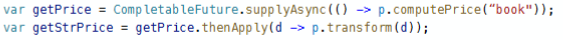
\includegraphics[width=0.8\linewidth]{Images/Future/thenapply.png}
\end{figure}